\chapter{Integrated Quantum Sources for Quantum Networks}
\label{ch:quantum-sources}

\section{From Photonic Devices to Network Components}

Quantum-secured networks depend on physical devices whose behavior must remain predictable after they leave a controlled laboratory setting. To build a robust quantum network, we must bridge the gap between idealized cryptographic protocols and the imperfect physical reality of the devices that implement them. Entangled-photon sources are one such foundational device class: they determine the spectral structure, brightness, purity, and long-term stability of the quantum states that later protocols consume. If these source properties drift with fabrication tolerances, thermal changes, or uncontrolled mode interactions, then the network layer inherits an unstable security and performance foundation.

This chapter begins the thesis body at the photonic-device layer. It examines dual-coupled micro-ring resonators as integrated sources for frequency-bin entangled photons. The common thesis-level question is not only whether such a device can generate useful quantum states, but whether it can be designed, tuned, and modeled in a way that makes it suitable for larger quantum--classical network systems.

\paragraph{Scope and assumptions.} This dissertation is a systems and networking contribution rather than a study of quantum-mechanical foundations. It assumes familiarity with the basic formalism of quantum states, measurement, entanglement, and the no-cloning theorem, and treats these as building blocks instead of deriving them; readers seeking that background are referred to standard texts~\cite{nielsen2010quantum}. For a deeper exploration of quantum optics, particularly concerning spatial modes and free-space optical communication, readers are referred to the author's prior work~\cite{meyer2024master}. The contributions reported here lie in how these primitives are designed, accelerated, stabilized, and integrated across the device, protocol, and infrastructure layers.

\section{Nonlinear Optics and Four-Wave Mixing}
\label{sec:qsrc-nonlinear}

The generation of entangled photon pairs in integrated photonics relies fundamentally on nonlinear optical processes. In centrosymmetric materials such as silicon and silicon nitride, the lowest-order nonlinear response is the third-order susceptibility, $\chi^{(3)}$. This nonlinearity mediates spontaneous four-wave mixing (SFWM), the process by which two pump photons are annihilated to create a signal and an idler photon pair.

Energy conservation dictates that the frequencies of the generated photons satisfy $2\omega_p = \omega_s + \omega_i$, where $\omega_p, \omega_s$, and $\omega_i$ are the pump, signal, and idler frequencies, respectively. Momentum conservation, or phase matching, requires that the propagation constants satisfy $2k_p = k_s + k_i + \Delta k$, where $\Delta k$ is the phase mismatch. In a microring resonator, phase matching is naturally achieved when the pump, signal, and idler fields align with the cavity resonances.

The efficiency of SFWM is highly dependent on the spatial overlap of the optical modes within the waveguide and the nonlinear refractive index of the material. Silicon nitride ($\text{Si}_3\text{N}_4$) has emerged as a leading platform for SFWM due to its ultra-low linear propagation loss, wide transparency window spanning from the visible to the mid-infrared, and absence of two-photon absorption at telecom wavelengths. These properties allow for the use of high-power continuous-wave pumps, maximizing the pair generation rate while maintaining high spectral purity.

By carefully engineering the waveguide cross-section, the group velocity dispersion (GVD) can be tailored to ensure broad phase-matching bandwidths. This dispersion engineering is critical for generating frequency-bin entangled states, where the signal and idler photons can occupy multiple pairs of symmetric resonance modes, creating a high-dimensional entangled state suitable for multiplexed quantum communication.

\section{Microring Entanglement Sources}
\label{sec:qsrc-microring}

Integrated photonics addresses the device-level bottleneck in deployable quantum
communication. Traditional tabletop optics, with discrete non-linear crystals and
mirrors, are too fragile, bulky, and expensive for wide-scale deployment. Photonic
integrated circuits (PICs) aim to miniaturize these components onto a semiconductor
chip using fabrication processes compatible with existing CMOS or telecom infrastructure.

For entanglement-based QKD and future repeater networks, the photon source is the critical component. It determines
the spectral structure, brightness, purity, and long-term stability of the photon pairs
that every subsequent protocol stage consumes~\cite{Wehner2018}. If a source emits
multiphoton pulses or indistinguishable spectral modes drift due to temperature fluctuations,
the visibility of quantum interference drops, the QBER rises,
and the protocol may fail to generate secure keys.

The work in this chapter focuses on microring resonators as candidate sources for
frequency-bin entanglement via spontaneous four-wave mixing (SFWM). In a microring,
light circulates and interferes constructively only at specific resonant frequencies
separated by the free spectral range (FSR). Key physics and engineering considerations
include:

\begin{itemize}
    \item \textbf{Quality Factor ($Q$):} A measure of the resonator's photon lifetime.
    High-$Q$ rings generate highly coherent, narrow-linewidth photons but are extremely
    sensitive to fabrication variations and thermal drift.
    \item \textbf{Thermal Tuning and Stability:} Refractive indices are temperature-dependent.
    Maintaining precise alignment with standardized telecom grids requires continuous,
    active thermal tuning, which can inadvertently affect the FSR and disrupt entanglement symmetry.
    \item \textbf{Spectral Purity (Schmidt Number):} A mathematically pure bipartite entangled
    state has a Schmidt number of 1. Real sources suffer from spectral correlations
    that degrade purity, necessitating precise dispersion engineering or tight filtering.
    \item \textbf{Platform Tradeoffs:} Silicon nitride ($\text{Si}_3\text{N}_4$) offers ultra-low
    loss and broad transparency but lacks the strong electro-optic (Pockels) effect of
    lithium niobate ($\text{LiNbO}_3$), meaning the choice of material dictates the tuning mechanisms
    available~\cite{Kumar2015,Mao2018,Grebenchukov2023}.
\end{itemize}

To provide the precise control required for networking, the dual-coupled architecture adds an auxiliary resonator to the main photon-pair generation ring. This additional degree of freedom can be used to reshape the spectral response of the source, compensate for nonidealities, and expose a control interface between device physics and network-facing metrics such as channel spacing, heralded purity, and Schmidt number. In this sense, the chapter treats source engineering as the first cross-layer problem of the dissertation: a physical-layer design choice must be made legible to the network and security layers built above it.

These device-derived quantities are precisely the parameters that determine the budget
available for coexistence with classical traffic. They define the point at which the
device layer becomes legible to the network layer above it.

\section{Source Characterization and Network Metrics}
\label{sec:qsrc-characterization}

Before an integrated quantum source can be deployed in a network, its performance must be quantified using metrics that translate directly to cryptographic utility. The raw generation rate of photon pairs is insufficient on its own; the quality of the entanglement and the distinguishability of the photons from background noise are paramount.

The primary figure of merit for the signal-to-noise ratio of a photon-pair source is the Coincidence-to-Accidental Ratio (CAR). It compares the rate of true coincident detection events (where both the signal and idler photons from a single pair are detected) to accidental coincidences (caused by dark counts, detector jitter, or uncorrelated photons from multi-pair emission). A high CAR is essential for maintaining a low quantum bit error rate (QBER) in the subsequent QKD protocol.

Another critical metric is the heralded single-photon purity. In entanglement-based protocols, the detection of an idler photon "heralds" the presence of the signal photon. If the source suffers from strong spectral correlations between the signal and idler, the heralded state will be mixed rather than pure, degrading the visibility of two-photon interference (such as the Hong-Ou-Mandel effect). The Schmidt number quantifies this purity: a Schmidt number of $1$ indicates a perfectly factorable, pure state. Dispersion engineering in microrings, as discussed in Section~\ref{sec:qsrc-nonlinear}, aims to minimize these correlations to approach ideal purity.

\section{Distance Scaling and Quantum Repeaters}
\label{sec:qsrc-distance}

While point-to-point QKD has been demonstrated over hundreds of kilometers, it faces a fundamental scaling limit. In classical optical networks, the exponential attenuation of light in standard telecom fiber is overcome using optical amplifiers (such as erbium-doped fiber amplifiers, or EDFAs) spaced every 80 to 100 kilometers. However, the no-cloning theorem strictly forbids the deterministic amplification of unknown quantum states. 

As a result, the key rate in a direct QKD link decays exponentially with distance. While state-of-the-art techniques like Twin-Field QKD (TF-QKD)~\cite{lucamarini2018overcoming} have pushed the maximum transmission distance past 800 kilometers~\cite{wang2022twinfield}, the resulting secure key rates at these extreme distances are often on the order of bits per second---insufficient for encrypting high-volume datacenter traffic. Figure~\ref{fig:qkd-distance-rate} summarizes this distance--rate tradeoff: state-of-the-art demonstrations cluster below the repeaterless bound, and only quantum repeaters restore favourable scaling at long distance.

\begin{figure}[htbp]
  \centering
  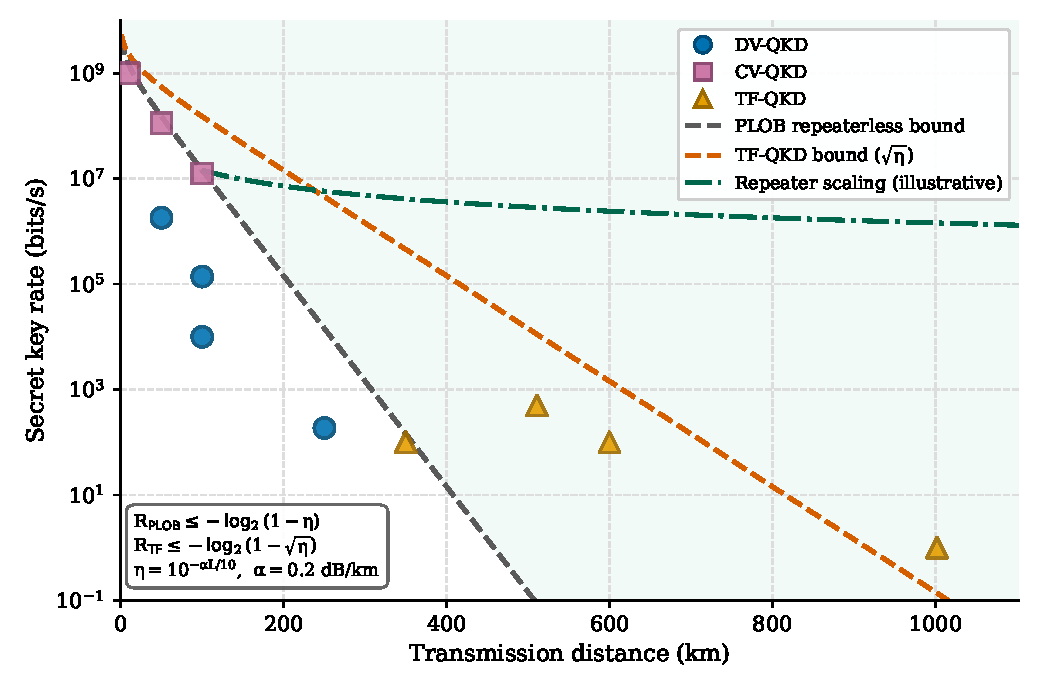
\includegraphics[width=\linewidth]{figures/chapter3/distance_keyrate.pdf}
  \caption[Distance scaling of QKD secret key rate]{Secret key rate as a
  function of transmission distance for quantum key distribution. In a direct,
  repeaterless link the secret key rate is fundamentally limited by the
  repeaterless Pirandola--Laurenza--Ottaviani--Banchi (PLOB)
  bound~\cite{pirandola2017fundamental} (grey dashed) and decays exponentially
  with distance.
  Twin-Field QKD improves the asymptotic scaling to $\sqrt{\eta}$ (vermillion
  dashed), extending reach beyond $1000$~km but only at rates of order bits per
  second. Restoring favourable, polynomial scaling at long distance requires
  quantum repeaters (green dash--dot, illustrative schematic), which lift the
  achievable rate into the shaded region above the PLOB bound. Markers show
  state-of-the-art WDM-compatible demonstrations (DV-, CV- and
  TF-QKD)~\cite{wang2025highrate,dynes2016ultrahigh,dolphin2023hybrid,ribezzo2023underwater,chen2021twinfield511,pittaluga2021repeaterlike,liu2023experimental1000,zhou2023twinfield};
  all lie below or near the repeaterless bound. Bounds assume standard $0.2$~dB/km fibre
  and a $1$~GHz reference clock; the repeater curve is illustrative, not
  measured.}
  \label{fig:qkd-distance-rate}
\end{figure}

To overcome this distance-rate tradeoff and achieve polynomial scaling, a global quantum network requires \emph{quantum repeaters}~\cite{briegel1998quantum}. Quantum repeaters divide a long-distance link into shorter, manageable segments. They operate by establishing entanglement across each short segment and then using entanglement swapping (a joint Bell-state measurement) to stitch these segments together, effectively teleporting the entanglement to the endpoints. 

The realization of quantum repeaters relies heavily on two components: quantum memories to store states until adjacent links succeed, and highly efficient, scalable sources of entangled photons to continuously populate the links. This necessity places immense pressure on the design of the photon sources: they must be bright, deterministic (or highly multiplexed), and spectrally compatible with the optical fibers carrying them.

\section{Coexistence with Classical Infrastructure}
\label{sec:qsrc-coexistence}

A further challenge for deploying quantum networks is the economic unfeasibility of laying dedicated ``dark fiber'' exclusively for quantum traffic. Practical quantum networking must co-exist with classical optical communications on the same fiber infrastructure using Wavelength Division Multiplexing (WDM). 

Integrating single-photon quantum channels alongside classical channels carrying milliwatts of power is notoriously difficult. The primary obstacle is spontaneous Raman scattering: the intense classical lasers scatter photons across a broad spectrum within the fiber, creating a noise floor that easily overwhelms the fragile quantum signals.

Overcoming Raman noise and achieving coexistence requires precise spectral filtering and alignment with the ITU telecom grid. The entangled photon sources must generate narrow-linewidth states at specific, standardized frequencies, and their emission characteristics must remain perfectly stable over time to allow ultra-tight filtering at the receiver. This requirement elevates the photon source from a physics experiment to a highly constrained network engineering component.

\section{Mapping Device Physics to Network Security}

The work in this chapter is written around the following mapping between low-level device behavior and the network requirements introduced in Chapter~\ref{ch:background}:

\begin{itemize}
  \item It addresses how quantum-secure networking primitives can be made compatible with deployed optical infrastructure. The focus is on C-band, wavelength-division-multiplexed operation and on resonator behavior that can be related to telecom channel plans~\cite{Kumar2015,Mao2018}.
  \item It addresses how low-level device parameters become system-level security constraints. Spectral purity, free spectral range stability, and the Schmidt number are device-derived quantities, but they influence interference visibility, quantum-bit error rate, and the practical budget available for coexistence with classical traffic~\cite{Grebenchukov2023}.
  \item It introduces the thesis pattern of cross-layer abstraction. Rather than treating a quantum source as a black box, the chapter asks which control variables and models are needed before a source can be used as a predictable component in a quantum network.
\end{itemize}

This chapter also sets up the transition to programmable network infrastructure in Chapter~\ref{ch:qkd-dpu}. The quantum source provides the raw optical resource, while later chapters ask how the resulting key material, cryptographic work, and observability tasks can be handled by DPUs, SmartNICs, and datacenter network systems.

\section{Contribution and Articles}

This chapter is built around two contributions that, taken together, move the dual-coupled microring (DCM) source from a promising integrated-photonics component toward a predictable network-engineering object. The author contributed to connecting the device studies to network requirements, the simulation-driven evaluation, and the thesis-level system interpretation; the experimental device work, modeling, and supervision were collaborative efforts with the co-authors.

The first contribution (P1), \enquote{Simulation-Driven Optimization of Dual-Coupled Micro-Ring Entanglement Sources for Quantum Optical Networks}, accepted to the 26th International Conference on Transparent Optical Networks (ICTON 2026), establishes the theoretical and modeling foundation for the chapter. It presents a coupled-mode-theory digital twin for the DCM source, relating auxiliary-cavity detuning, inter-ring coupling, and dispersion to photon-pair purity, brightness, and Schmidt number. By mapping low-level physical parameters to network-facing metrics, it defines the optimization space required to engineer quantum sources for specific network applications.

The second contribution (P2), \enquote{Free Spectral Range Stability under Linear Thermal Tuning in a Dual-Coupled Microring Resonator}, presented at the 2026 International Conference on Science and Electrical Engineering (ICSEE), provides the experimental validation of the device's stability. While the first paper demonstrated how the source can be optimized in simulation, this work grounds those findings in physical reality. Its key role is to show that thermal tuning of the auxiliary resonator---a necessary control mechanism---preserves the predictable free spectral range behavior required for channelized quantum network operation.

Together, the two papers establish that source behavior can be modeled, optimized, and physically stabilized in terms that later network layers can consume. This matters because quantum-secure communication is often limited by interfaces between layers: physical devices expose imperfect states; protocols assume idealized state properties; network planners allocate wavelengths and power budgets; and operators need stable, remotely configurable behavior. The resulting thesis claim is deliberately bounded. The chapter does not demonstrate a complete deployed quantum network, nor does it by itself close the practical-security gap of QKD systems; it establishes a modelable, stabilizable source as the foundation on which the rest of the thesis builds.

Two limitations should remain visible in the final dissertation. First, predictive source models must be continuously validated against fabricated devices across process variation and environmental drift; a digital twin that is not tied back to measurement risks becoming another idealized model. Second, source optimization is only one part of system security. Higher purity and stable channel spacing can improve the assumptions available to entanglement-based protocols, but coexistence noise, detector behavior, post-processing, authentication, and operational monitoring still determine whether a practical system remains secure~\cite{Xu2020}. These limitations motivate the rest of the thesis, which follows quantum-secure networking beyond the photonic source and into programmable post-processing, cryptographic acceleration, datacenter transport behavior, and confidential-AI observability. The immediate next step, in Chapter~\ref{ch:qkd-dpu}, moves from generating quantum-secure optical resources to processing the classical information that such systems produce on programmable network hardware.

\includedpaper{P1}{Simulation-Driven Optimization of Dual-Coupled Micro-Ring Entanglement Sources for Quantum Optical Networks}{meyer2026icton}{source-materials/papers/camera-ready/dcm-entanglement-sources-quantum-networks-camera-ready.pdf}

\includedpaper{P2}{Free Spectral Range Stability under Linear Thermal Tuning in a Dual-Coupled Microring Resonator}{meyer2026icsee}{source-materials/papers/camera-ready/fsr-stability-dual-coupled-microring-camera-ready.pdf}
